\chapter{\label{chap:nn-in-cv}Neural Networks in Computer Vision}

Machine learning (ML) is playing a great role in solving many tasks proposed by the field of computer vision (CV). Analyzing objects from images is task widely considered as not definable by a set of conditions and therefore, some sort of artificial intelligence (AI) has to be used, as is further discussed in Section~\ref{sec:ml}. When problems got more complicated, ML models had to be increased in depth, which led to introducing the term deep learning (DL). 

Neural networks (NNs) became a very powerful computing architecture in machine learning. Section~\ref{sec:cnn} informs how introduction of convolutional layers to neural networks further increased their efficiency in image processing. Various other operations were also implemented into convolutional neural networks (CNNs) to fit the needs of specific CV challenges.

Deep learning has untangled many problems which were not solvable with other methods. Recognition, being one of these problems, requires large amount of training data when the model is using supervised learning. This matter is further described in Section~\ref{sec:supervised}. The quality of annotated data  available for the training process has a great influence of the model performance and as such became a challenge in further development of recognition models.

Therefore, learning algorithms that do not require large datasets are being developed. One of these approaches is self-supervised learning introduced in Section~\ref{sec:self-supervised}. It extensively uses large amount of data without any labels as these are easier to obtain. Model trained in this manner needs a smaller amount of annotated data to generalize. Such attribute is very valuable since labeling can often be done only by hand and is very time consuming.

\section{\label{sec:ml}Machine Learning}

Computers are very good at solving problems that can be specified with a set of conditions and states, such as game of chess. The computational power that it possesses allows it to analyze the game many steps ahead. Whereas human mind finds these tasks very complicated. It is therefore no surprise that computers managed to defeat the best chess players in the world. That is why one of the ways to create an artificial intelligence (AI) focused on knowledge base approach. The main hypothesis was that every problem can be described in a formal language. After designing a set of logical inference rules, the problem would be solved with just a simple inference.

Unfortunately, when it comes to solving real world problems, this approach cannot be applied. Humans have immense knowledge about the world and applying it is very subjective and intuitive. It cannot be formalized in any way. The knowledge base AI often did not understand the problem correctly and provided misleading results. Another disadvantage is that the formalization itself was an unwieldy process requiring a large amount of human staff \cite{Goodfellow-et-al-2016}.

Different approach had to be chosen to solve real world tasks. Instead of modeling the real world with conditions and rules, a probabilistic models with a set of parameters were chosen. Most parameters are to be set automatically based on the data provided to learn the problem's nature. Logistic regression is one these basic models that provides subjective reasoning based on the information that it learned from previous real world examples. It finds correlation between inputs and various outcomes. The computation involves weighted sum of the inputs and non-linear transformation of this sum. Parameters that are adjusted are the weights of each input and a bias, single number that is added to the sum, which can be also seen as a weight to a constant input of $+1$. 

Inputs of these models are called features of the data and the performance of the model heavily depends on their representation. If the features correlate with the different outcomes, model is expected to provide good results. If we wanted to recognize a sports pose and the data provided would be positions of all joints and both eyes in a human body, the task would be fairly easy. After normalizing the scene to always have the same scale and point straight to the eyes, the task gets even simpler. Inputs of such model would be coordinates of mentioned objects and outputs probabilities of each sports pose. This solution introduces another a lot more complicated challenge -- the coordinates are hard to obtain without any special tools. What we would like to have is a model that can work on simple image data since obtaining those is affordable.

Images can be described with pixel values and provided to the input but individual pixels have no direct correlation to sports poses, therefore, the predictions would be useless. There are number of examples why this is true but perhaps the easiest one is translational dependence. Having the sports pose moved just few pixels in any direction from where it is expected to be makes the results incorrect. Additional problems would be caused by shadows, different clothes that the person is wearing etc.

This obstacle can be overcome by having the ML model discover not only mapping of features to outputs but also finding the useful features in the raw data on its own. This makes the model not only work on raw data but also generalizes it to different tasks. For example not only recognizing sports poses but also vehicles with the same model only trained on different data. Logistic regression is not capable of doing such predictions, some more complex solution has to be found. In computer science, concept of building complex structures from simple modules is well known and can be used in machine learning as well. By combining many logistic regressions into a structure, neural network (NN) is created \cite{Goodfellow-et-al-2016}.

These networks consist of neurons -- logistic regressions. Its non-linear function can be adjusted to fit the needs of a specific task and it is often referred to as activation function. The capability to solve complex problems arises from structuring of simple neurons into groups called layers, illustrated in Figure~\ref{fig:network-with-neuron}. The key is not doing the mapping of abstract features in one task but dividing it into multiple simple mappings. The input layer, also called visible layer because its data can be easily observed, provides data to the following layer. First simple mapping is done by the second layer and each following layer uses the mappings of its predecessor to obtain more complex information from the data. These following layers are also called hidden because their values are not given in the data, they have to be determined by the model. Finally, the last layer provides outputs in a format specified by its activation function.

\begin{figure*}[ht]\centering
    \centering
    \includegraphics[scale=0.55]{figures/neural_network_with_neuron.ai}
    \caption{Neural network with densely connected neurons and detailed explanation of one of them. Every neuron computes a simple weighted sum and non-linear operation on a set of inputs. Inputs are obtained from the previous layer or the raw data itself and outputs are then send to neurons in the following layer. No neurons cooperate with others in the same layer.}
    \label{fig:network-with-neuron}
\end{figure*}

With tasks becoming more complicated, the number of layers is growing bigger. As there was increase in the depth of the graph, such networks were called deep neural networks and their usage was referred to as deep learning (DL).

Neural network for classification can be seen as function $\pmb y=f(\pmb x | \pmb \theta)$ that maps input vector $\pmb x$ to a category $\pmb y$ with parameters of the network given by $\pmb \theta$. It is also possible to decompose the neural network function $f$ to multiple functions, each one representing one layer, applied in the correct order. NN with two hidden layers $f^{(1)}$, $f^{(2)}$ and one output layer $f^{(3)}$ is representing function:

\begin{equation}
    \label{eq:forward-prop}
    \pmb y = f(\pmb x) = f^{(3)}(f^{(2)}(f^{(1)}(\pmb x))).
\end{equation}

Network parameters $\pmb \theta$ are basically weights and biases of each neuron and they are unknown when the model is constructed. The ideal values of parameters cannot be computed in a simple way because of non-linearity of neural networks that causes most of the loss functions to become non-convex. Loss functions are going to be further explained later in this section. NN parameters have to be somehow initialized and iteratively improved to provide better results. This iterative process is called learning or training and its goal is to approximate some function $f^*$ that provides accurate results for given problem. That is achieved by finding parameters $\pmb \theta$ that result in such approximation \cite{Goodfellow-et-al-2016}.

Non-linear results of neural networks are achieved with activation functions. There are lots of various functions with different use cases, but two of them are very common. One is a sigmoid function with Equation~\ref{eq:sigmoid}, which maps any real number to a number between 0 and 1. It is often used to represent probability. The other activation function is rectified linear unit (ReLU) (Equation~\ref{eq:relu}) that is linear for any positive number and 0 otherwise. ReLU is very often used in later discussed convolutional neural networks.

\begin{equation}
    \label{eq:sigmoid}
    \sigma (x) = \frac{1}{1 + e^{-x}}
\end{equation}

\begin{equation}
    \label{eq:relu}
    f(x) = \max(0, x)
\end{equation}

Learning algorithm consists of multiple stages that repeat until the model is producing satisfactory results. These stages are explained into detail in following paragraphs.

\begin{enumerate}
    \item Forward propagating data -- inference.
    \item Computing gradients with back-propagation algorithm.
    \item Calculating learning rate.
    \item Performing learning step of the model with optimization algorithm.
\end{enumerate}

Evaluation $\pmb y$ of samples $\pmb x$ is computed by forward propagating the samples through the network. That means evaluating all layers in the correct order as illustrates Equation~\ref{eq:forward-prop}. Correct values $\pmb y^*=f^*(\pmb x)$ are known because the training data are annotated with them. Loss (or cost) function can be used to compute how good the approximation $f$ of $f^*$ is. Loss functions are designed to fit specific tasks and data distribution. When it is necessary to compute some sort of distance on data that probably come from Gaussian distribution, Mean Squared Error function is often used.

For classification problems, the typical choice is a measure called cross-entropy. It is based on the Kullback Leibler divergence, which measures the difference between two probability distributions. Cross-entropy computes the expected number of bits needed to represent data coming from distribution $p$ while using the distribution $q$ and it is calculated as follows \cite{pml1Book}:

\begin{equation}
    \label{eq:cross-entropy}
    \mathbb{H}(p, q) \triangleq -\sum\limits_{y} p(y) \log q(y).
\end{equation}

Gradients can be computed in many different ways but the most common one for models that are working on large datasets is stochastic gradient descent (SGD). Therefore, this is the only one discussed in this thesis. Generally, gradient is a vector pointing in the direction of steepest ascent. By following such vector, local maximum can be reached. In machine learning, the thought is often reversed -- the goal is to reach local minimum, but the main idea remains the same. For number of samples $m$ and loss function $L$, gradient $\pmb g$ is computed with this equation: 

\begin{equation}
    \label{eq:sgd}
    \pmb g = \frac{1}{m} \sum\limits_{i=1}^{m} \nabla_{\pmb \theta} L(f(\pmb {x}^{(i)}| \pmb \theta), {y}^{*(i)}).
\end{equation}

The direction of next step is computed but another variable called the learning rate is still unknown. It represents the size of the step and it has a vast impact on the training performance. One possible solution is to keep the learning rate fixed for the whole training but better results can be achieved with more advanced algorithms. First improvement can be achieved by computing a specific learning rate for each parameter of the network. The second way to achieve better results is by changing the learning rate throughout the training process.

The update of parameters is done with an optimization algorithm. It uses previously computed gradient $\pmb g$ and other algorithm specific parameters to update the network's parameters. It usually incorporates the calculation of learning rate. Very common is use of Adam optimization algorithm that also uses the previously mentioned improvements for more useful learning rate. The algorithm uses mean and uncentered variance of parameters to adapt the learning rates. The computation goes as follows \cite{kingma2017adam}.

\begin{equation}
    \pmb s = \rho_1 \pmb s + (1 - \rho_1) \pmb g
\end{equation}

\begin{equation}
    \pmb r = \rho_2 \pmb r + (1 - \rho_2) \pmb g \odot \pmb g
\end{equation}

\begin{equation}
    \hat{\pmb s} = \frac{\pmb s}{1 - \rho_1}
\end{equation}

\begin{equation}
    \hat{\pmb r} = \frac{\pmb r}{1 - \rho_2}
\end{equation}

\begin{equation}
    \Delta \pmb \theta = - \epsilon \frac{\hat{\pmb s}}{\sqrt{\hat{\pmb r}} + \delta}
\end{equation}

\begin{equation}
    \pmb \theta = \pmb \theta + \Delta \pmb \theta
\end{equation}

\noindent Where:

$\rho_1, \rho_2$ are exponential decay rates for moment estimates (mean and variance, usually initialized to 0.9 and 0.999 respectively),

$\odot$ is an element-wise product,

$\pmb s$ is an updated biased first moment estimate,

$\pmb r$ is an updated biased second moment estimate,

$\hat{\pmb s}$ is a correct bias in the first moment,

$\hat{\pmb r}$ is a correct bias in the second moment,

$\epsilon$ is a step size (usually initialized to 0.001) and

$\delta$ is a small constant used for numerical stabilization (usually initialized to $10^{-8}$).

\vspace{0.2cm}

Another important part of the training process is how the data samples are handled. It is possible to update network's parameters after with each sample but also with the whole dataset. The ideal solution is to divide dataset into minibatches of size ranging from lower tens to higher hundreds of samples. Parameters are then update with each minibatch. After all minibatches of the dataset has been used for training, the process can start again on the previously minibatches. It is also important to shuffle the data in the dataset and in the minibatches. If the same order of samples was used, the network might have problems with not generalizing enough.

Every time the whole dataset has been handled, one epoch has passed. Training can consist of many epochs, depending on the problem difficulty, network size and dataset. It is important to measure the network's performance on data it has never seen during the training. Once model's accuracy is not improving and/or loss is approaching nearly zero values, the training will no longer provide better results. Therefore, dataset should be divided into training and validation data.

\section{\label{sec:cnn}Convolutional Neural Networks}

Convolutional neural networks are a special kind of NNs including at least one layer that is computing convolution. These networks are used for processing of data with grid-like topology, such as sequences and images. This thesis focuses on image data and therefore, only those will be discussed further on, even though the computation can be generalized to other input types.

At first, convolution is discussed as an operation on image data with its important properties. Its usage as a layer in neural network is explained into detail. Then, other operations important for CNNs are introduced and explained. Once most of the important principles of convolutional neural networks have been mentioned, a specific convolutional neural network architecture is presented.

\subsection{\label{sec:conv-on-image}Convolution on Image Data}

Convolution is a mathematical operation of two functions that produces a third function that describes how one modifies the other in shape. This is a very general definition that is not necessary for image processing and can be made more specific. It is only necessary to consider discrete values of inputs, continuous functions are not used in CNNs. Images usually consist of multiple channels (typically red, green, and blue), but for convolutional neural networks, channels are handled separately. For that reason, images will be discussed as a 2-dimensional arrays of numbers only.

Convolution computes a weighted sum of values across a fixed-size area of the image. It takes a 2-D image input and 2-D array of weights called kernel. Images can be extended on the edges with padding, which are basically pixels with value zero. Since convolution changes the size of the input image, padding is often used to equalize the sizes \cite{dumoulin2016guide}. Resulting 2-D array is often referred to as a feature map and it is computed by multiplying input value with corresponding kernel value for all of the overlapping elements and then summed together. After that, kernel moves one step further on the input and next value of the feature map is calculated the same way, until the whole input is processed. Figure~\ref{fig:convolution} illustrates ho.

\begin{figure*}[ht]\centering
    \centering
    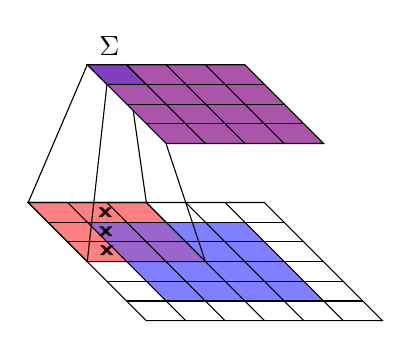
\begin{tikzpicture}[scale=1]
        \fill[fill={rgb:blue,1;white,1}] (1, 0) -- (3, 0) -- (2, 1) -- (0, 1) -- cycle;
        \draw[fill={rgb:red,1;white,1}] (0, 0.5) -- (1.5, 0.5) -- (0.75, 1.25) -- (-0.75, 1.25) -- cycle;
        \fill[fill={rgb:red,1;blue,2;white,2}] (0.5, 0.5) -- (1.5, 0.5) -- (1, 1) -- (0, 1) -- cycle;
        \draw (0.75, -0.25) -- (3.75, -0.25) -- (2.25, 1.25) -- (-0.75, 1.25) -- cycle;
        \draw (0.5, 0) -- (3.5, 0);
        \draw (0.25, 0.25) -- (3.25, 0.25);
        \draw (0, 0.5) -- (3, 0.5);
        \draw (-0.25, 0.75) -- (2.75, 0.75);
        \draw (-0.5, 1) -- (2.5, 1);
        \draw (1.25, -0.25) -- (-0.25, 1.25);
        \draw (1.75, -0.25) -- (0.25, 1.25);
        \draw (2.25, -0.25) -- (0.75, 1.25);
        \draw (2.75, -0.25) -- (1.25, 1.25);
        \draw (3.25, -0.25) -- (1.75, 1.25);
        
        \draw (0, 0.5) -- (0.25, 2.75);
        \draw (1.5, 0.5) -- (0.75, 2.75);
        \draw (0.75, 1.25) -- (0.5, 3);
        \draw (-0.75, 1.25) -- (0, 3);
        
        \draw[fill={rgb:red,1;blue,1;white,1}] (1, 2) -- (3, 2) -- (2, 3) -- (0, 3) -- cycle;
        \draw[fill={rgb:red,1;blue,2;white,1}] (0.25, 2.75) -- (0.75, 2.75) -- (0.5, 3) -- (0, 3) -- cycle;
        
        \node [xshift=8,yshift=92] {$\Sigma$};
        \node [right=-0.6, yshift=32] {\scriptsize$\times$};
        \node [right=-0.1, yshift=32] {\scriptsize$\times$};
        \node [right=0.4, yshift=32] {\scriptsize$\times$};
        \node [right=-0.4, yshift=25] {\scriptsize$\times$};
        \node [right=0.1, yshift=25] {\scriptsize$\times$};
        \node [right=0.6, yshift=25] {\scriptsize$\times$};
        \node [right=-0.1, yshift=18] {\scriptsize$\times$};
        \node [right=0.4, yshift=18] {\scriptsize$\times$};
        \node [right=0.9, yshift=18] {\scriptsize$\times$};
        
        \draw (0.25, 2.75) -- (2.25, 2.75);
        \draw (0.5, 2.5) -- (2.5, 2.5);
        \draw (0.75, 2.25) -- (2.75, 2.25);
        \draw (0.5, 3) -- (1.5, 2);
        \draw (1, 3) -- (2, 2);
        \draw (1.5, 3) -- (2.5, 2);
    \end{tikzpicture}
    \caption{Example of 2-dimensional convolution with input size 4 (blue), kernel size 3 (red) and padding size 1 (white). Feature map (dark purple) has the same size as input because of the padding.}
    \label{fig:convolution}
\end{figure*}

The operation of convolution is often denoted with an asterisk $*$ and for input $I$ of size $m \times n$ and kernel $K$, feature map $FM$ is calculated as:

\begin{equation}
    FM(i, j) = (I * K)(i, j) = \sum\limits_m \sum\limits_n I(m, n) K(i-m, j-n).
\end{equation}

Layers that perform convolution are not that different from normal dense layers mentioned in the previous section. Input image is the layer's input, weights are the kernel values and output of the layer is the feature map. When training is performed, the goal is to find kernel values that produce the best results. Kernels are usually called filters in CNN context, therefore, this terminology will be used from now on. Each convolution layer often includes more filters and produces the equal number of feature maps, one feature map from each filter applied to the input. That means 2-D input data are transformed into 3-D data, as there are multiple 2-D feature maps of the same size. Following convolution layer applies filters to each input and sums the results over each filter. Color images on the input are handled the same way as if each channel was a feature map from a previous convolution layer, there is no difference between them.

Convolution is a very important operation for image processing because it holds many essential properties. Since it is computed over multiple neighboring values, context of pixel values is taken into account, not just the single values. That enables pattern recognition in images. Simple patterns as shadow information and edges are layer by layer combined into more complex patterns, until an object detection can be done. Another important property is equivariance, which means that position of objects in the image plays no role in detection. Finally, convolution has low memory requirements that are not dependant on input size, only values that are stored are 2-D filter arrays \cite{Goodfellow-et-al-2016}.

\subsection{\label{sec:other-cnn-ops}Additional Important Parts of Convolutional Neural Networks}

Convolution layers are usually followed by \textit{pooling} layers in CNN architecture. Pooling is a function that for each value of the input grid computes a summary statistic of its nearby values. The most common statistics are maximum and average. For example, max pooling layer with $2 \times 2$ pool size takes a maximum of every $2 \times 2$ region in the image and creates a new image constructed out of the maximum values. In this case, output size will be smaller than input size. To keep the size uniform, padding must be added the same way it was added during convolution.

\begin{figure*}[ht]\centering
    \centering
    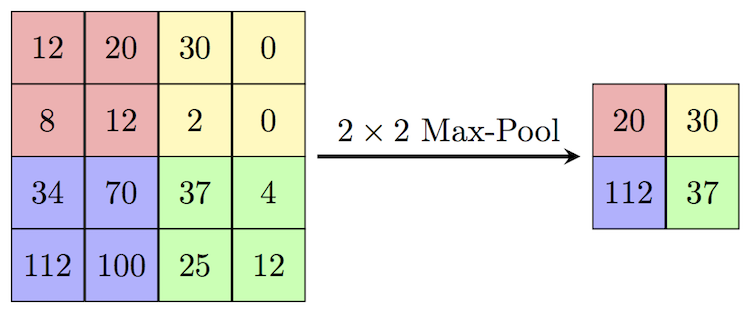
\includegraphics[]{figures/todo-maxpool.png}
    \caption{Example of max pooling \todo{change for own vector illustration}.}
    \label{fig:pooling}
\end{figure*}

Pooling layers make the model invariant to small translations. Even when the input has moved few pixels in some direction, pooled outputs should not change much. Pooling can be also easily used for downsampling of images when stride is set to 2 or more. Another use case of pooling is handling images of varying size because classifiers are accepting only images with fixed size \cite{Goodfellow-et-al-2016}.

\textit{Inception} modules introduce a couple of important concepts to CNN architecture. They perform multiple pooling and convolutions with multiple kernel sizes on one spatial input (e.g. multiple feature maps from previous convolution layer). Resulting new feature maps are depth-concatenated to keep output in a general 3-D format. Convolutions and pooling are done with correct padding to keep width and height of feature maps identical. The inception module is illustrated in Figure~\ref{fig:inception} with its key concepts explained in following paragraphs \cite{szegedy2014going}.

\begin{figure*}[ht]\centering
    \centering
    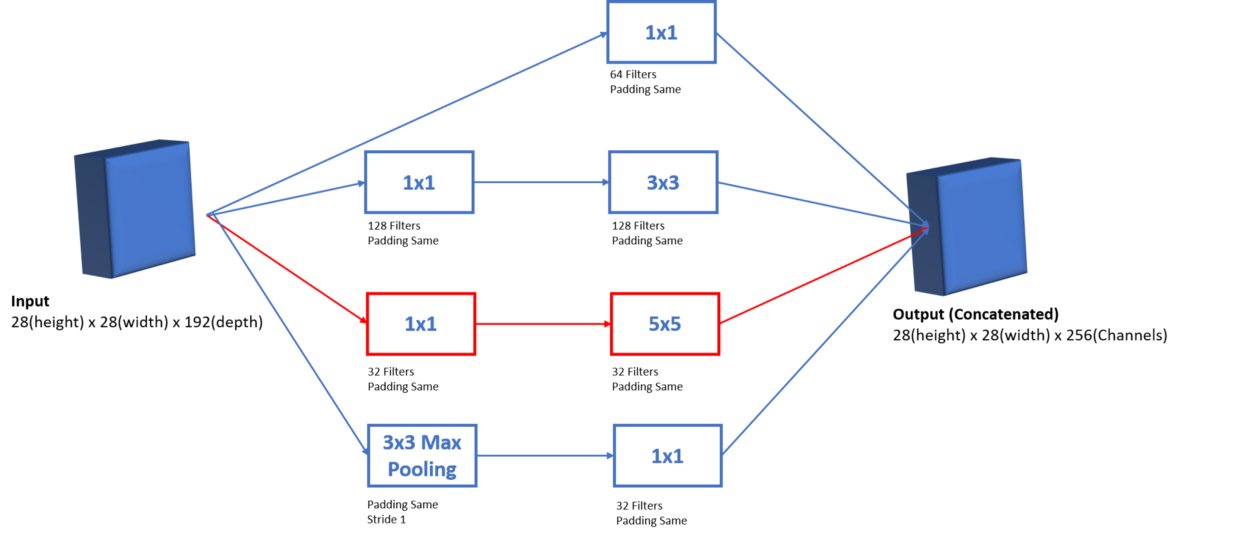
\includegraphics[scale=0.3]{figures/todo-inception.png}
    \caption{Inception module \todo{change for own vector illustration}.}
    \label{fig:inception}
\end{figure*}

Convolution layer with filters of size $1 \times 1$ keeps the width and height of input the identical but they change the depth of it. With different number of filters than what is the depth of the image, this layer is able to learn patterns across different feature maps. While pooling layer is useful for width and height reduction of the input, 1x1 convolution layer can reduce the input in depth.

Inception modules also consist of the convolution layers with filter sizes $3 \times 3$ and $5 \times 5$. Their goal is capturing the spatial patterns of input -- height, width, and also depth. Problem of these layers is that they are computationally demanding, but this can be solved if they are preceded by previously mentioned $1 \times 1$ convolution layer. By first reducing the depth of the input and then performing the same operation, lower number of operations is performed while still keeping the great performance of multiple convolutions.

\textit{Residual blocks} made a vast impact on the development of convolution neural networks. While the recognition problems got more complicated and datasets enormous, the need to make CNNs deeper arose. Unfortunately, performance of the networks did not improve with just adding more layers. Gradients could not be back-propagated all the way to initial layers.

Solution of this problem came with residual blocks that introduced a simple connection that bypassed blocks with convolution and pooling, as shown in Figure~\ref{fig:residual}. This connection symbolizes a simple identity function, it takes the input and outputs it unchanged. When such identity connection bypasses every convolution block, the neural network can basically work as an identity function. The same principle can be applied when gradients are computed, therefore, larger gradients are back-propagated to the initial layers \cite{he2015deep}.

\begin{figure*}[ht]\centering
    \centering
    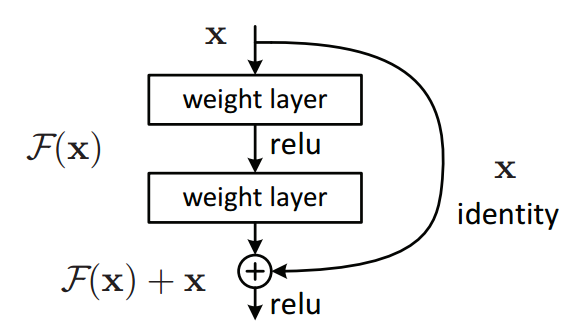
\includegraphics[scale=0.3]{figures/todo-residual.png}
    \caption{Residual block \todo{change for own vector illustration}.}
    \label{fig:residual}
\end{figure*}

\textit{Dropout} layer is used to deactivate some neurons during the training process and by that, it is trying to simulate different models. For each mini-batch of data, some percentage of neurons have their activation function set to zero. The training step is done as usual -- inference, back-propagation and weight update. Then, for the next mini-batch, different neurons are chosen to produce output with value zero. Dropout is a computationally inexpensive way to regularize models \cite{Goodfellow-et-al-2016}.

\todo{Consider adding depth-wise convolutions (MobileNet).}

\todo{Consider adding self-attention (CoAtNet) -- pretty complicated tho.}

\section{\label{sec:supervised}Recognition as a Supervised Learning Task}

Recognition is one of many computer vision tasks and it can be further divided into multiple more specific categories. The most common one is classification -- the recognized image is supposed to be assigned a class from previously known set. This thesis focuses specifically on sports poses classification, however, the other recognition varieties are worth mentioning as well. Detection and segmentation challenges are trying to localize objects in images with bounding box or pixel-wise, respectively. Very specialized task is pose estimation where the model is trying assign a specific structure of connected joints to a human body.

Supervised learning is one of the most general training methods. The main prerequisite is generally dataset with annotated samples. For classification task, each data point has to have a class assignment. During the training procedure, the model is trying to assign the correct class to each sample in a mini-batch and compare it to ground truth -- the real class of the sample saved in the dataset. If the model is not successful, the information is back-propagated through the network to improve on the next mini-batch inference.

Nowadays, models are trained on datasets of millions or even billions of data points. Networks with number of layers well over 100 have enough parameters to be able to classify very complicated images to a large number of categories (even tens of thousands hierarchically divided ones). Important property of each classifier is its ability to generalize -- to classify correctly images it has never seen. Generalization is achieved with training on immense datasets with large variety of images.

\subsection{State-of-the-Art Models for Recognition}

\todo{Choose architecture that will be first explained and then shown below.}
\blindtext

\todo{If CoAtNet is chosen, self-attention should be covered in the theoretical section -- it is the true SOTA right now.}

\todo{If MobileNet is chosen, depth-wise convolution should be covered in the theoretical section -- will be probably used in the code.}

\todo{If ResNeXt is chosen, everything should be theoretically covered -- is nice as an illustration of some key concepts.}

\begin{figure*}[ht]\centering
    \centering
    
\includegraphics[width=\linewidth,height=1.5in]{figures/placeholder.pdf}
    \caption{Example of Convolutional Neural Network architecture.}
    \label{fig:cnn-example}
\end{figure*}

\blindtext

\blindtext

\blindtext

\blindtext

\subsection{Current Advances in Sports Pose Recognition}

Most of the current research focuses on sports pose estimation which is a different task than sport pose classification done in this thesis. Researchers also tried yoga pose recognition from body contours but the variety of poses did not draw near to all possible options \cite{yoga-posture-recognition}. However, with publishing of Yoga-82 dataset, results of different supervised-trained models were also analyzed \cite{verma2020yoga}. Summarized in Table~\ref{tab:yoga82-results} are the results of classifying images from Yoga-82 dataset with various CNN models.

\begin{table}[ht]
    \centering
    \begin{tabular}{l r r r r}
        \hline
        Architecture & Depth & Parameters & Top-1 Accuracy & Top-5 Accuracy \\
        \hline
        ResNet-101 & 101 & 42.72 M & 65.84 & 84.21 \\
        DenseNet-169 & 169 & 12.60 M & 74.73 & \textbf{91.44} \\
        DenseNet-201 & 201 & 18.25 M & \textbf{74.91} & 91.30 \\
        MobileNet-V2 & 88 & 2.33 M & 71.11 & 88.50 \\
        ResNeXt-50 & 50 & 23.15 M & 68.45 & 86.42 \\
        \hline
    \end{tabular}
    \caption{Performance of widely-known CNN architectures on Yoga-82 dataset using third-level classes from \cite{verma2020yoga}.}
    \label{tab:yoga82-results}
\end{table}

Yoga-82 dataset contains 82 third-level classes of yoga poses grouped into 20 second-level classes that are further merged into 6 first-level classes. The poses are grouped according to the posture and pose look. Of course, not all poses can be easily assigned one of the 82 third-level classes, some variation has to be taken into account. Hierarchy of classes can be used to improve the classification or to estimate a pose type with higher accuracy -- reported first, second, and third-level accuracy is $89.81\,\%$, $84.59\,\%$, and $79.08\,\%,$ respectively, for top-1 accuracy on DenseNet-201.

Yoga as a sport includes an extensive amount of poses with variety that stands out amongst other sports. The poses can be also sorted into groups and thus create a hierarchy that can be further used for classification as can be seen in \cite{verma2020yoga}.

\section{\label{sec:self-supervised}Self-Supervised Learning for Computer Vision}

Self-supervised learning is a method of training a model first to learn data representations on unannotated data and then to use annotated data to train another model for classification on the representations. The first model learns patterns in the data and how to represent the needed information in it with a latent vector. There is no need for any labels since the data itself is used for supervision. Means of obtaining the supervision differ upon the task and data available. The second model needs to use annotated dataset to assign classes to latent vector output by the first model. Classification is made easier with the data being represented efficiently and there is no need for large annotated datasets to achieve a good generalization properties of the model.

There are various ways to use the image data itself as a supervision. For instance, it is possible to use a small distortion on the original data and expect it to not change its meaning. With this, different images that are bind together are created automatically. Self-supervision can also be used for colorization tasks, the original color images are easily converted into grayscale images and the model's goal is to colorize it to match the original sample. Another common challenge is generating missing image data, which is done with context encoders. Some part of the image is cropped out and the encoder is trying to fill it in to the previous form.

This thesis uses models called time-contrastive networks (TCNs) introduced in \cite{sermanet2018timecontrastive}. Self-supervision is achieved with using multiple cameras to film a scene from different viewpoints, Figure~\ref{fig:multiple-viewpoints} displays such setup. After the videos are synchronized, frames with the same timestamp but from different cameras should still produce latent vectors fairly close to each other. When the timestamps are different (and the scene changed), latent vectors should be further from each other even when filmed from the identical viewpoint.

\begin{figure*}[ht]\centering
    \centering
    
\includegraphics[width=0.5\linewidth,height=1.5in]{figures/placeholder.pdf}
    \caption{\todo{Scene from multiple viewpoints.}}
    \label{fig:multiple-viewpoints}
\end{figure*}

Self-supervised models use different loss functions that suit their specific approach to solving the problem. As described in the previous paragraphs, self-supervised learning has many different forms and, therefore, architectures vary in many ways. Time-contrastive network has to learn to represent the object in the image independently on the viewpoint. Images from the same viewpoint can differ just a little in time but their image embeddings should be different if the observed object changed. Whereas images from different viewpoints at the same time can be entirely different, only the observed object is constant. Therefore, their embeddings should be reasonably similar. Such challenge can be solved with loss function called the triplet loss.

\subsection{Triplet Loss Function}

Triplet loss function pushes embeddings of similar data closer together and pulls embeddings of diverse data further apart. Its main goal is learning data representation in a $d$-dimensional Euclidean space. Inputs of the function are 3 data embeddings -- anchor, positive, and negative. Anchor and positive should be closer to each other than anchor and negative. It can be thought of as anchor and positive belonging to the same class and negative to a different one \cite{facenet-triplet-loss}.

Data point $x$ has an embedding $f(x) \in \mathbb{R}^d$ which is additionally constrained to live on a unit hypersphere -- ${|| f(x) ||}_2 = 1$. Triplet $i$ consists of anchor image $x^{a}_{i}$, positive image $x^{p}_{i}$ and negative image $x^{n}_{i}$. The goal of the network is for inequality  \ref{eq:triplet-distance} to held true with condition \ref{eq:triplet-condition}.

\begin{equation}
    \label{eq:triplet-distance}
    {|| f(x^{a}_{i}) - f(x^{p}_{i}) ||}^{2}_{2} + \alpha < {|| f(x^{a}_{i}) - f(x^{n}_{i}) ||}^{2}_{2}
\end{equation}

\begin{equation}
    \label{eq:triplet-condition}
    \forall ( f(x^{a}_{i}), f(x^{p}_{i}), f(x^{n}_{i})) \in \mathcal{T}
\end{equation}

\noindent Where $\alpha$ is a margin that is enforced between positive and negative pairs and $\mathcal{T}$ is the set of all possible triplets, $|\mathcal{T}| = N$.

The triplet loss to be minimized is then:

\begin{equation}
    \label{eq:triplet-loss1}
    L = \sum\limits^{N}_{i}
    \left[
    {|| f(x^{a}_{i}) - f(x^{p}_{i}) ||}^{2}_{2} - {|| f(x^{a}_{i}) - f(x^{n}_{i}) ||}^{2}_{2} + \alpha
    \right]_{+}.
\end{equation}

\noindent And more often it is used as:

\begin{equation}
    \label{eq:triplet-loss2}
    L = \sum\limits^{N}_{i}
    \max{(0, {|| f(x^{a}_{i}) - f(x^{p}_{i}) ||}^{2}_{2} - {|| f(x^{a}_{i}) - f(x^{n}_{i}) ||}^{2}_{2} + \alpha)}.
\end{equation}

The triplet selection is an important part of the whole training process. When the constraint \ref{eq:triplet-condition} is easily met, the triplet has not improved the model at all and therefore, it will converge slower. The ideal triplets (hard positive and hard negative, respectively) are satisfying these two conditions \cite{facenet-triplet-loss}:

\begin{equation}
    \label{eq:triplet-sel1}
    \argmax_{x^{p}_{i}}{{|| f(x^{a}_{i}) - f(x^{p}_{i}) ||}^{2}_{2}},
\end{equation}

\begin{equation}
    \label{eq:triplet-sel2}
    \argmin_{x^{n}_{i}}{{|| f(x^{a}_{i}) - f(x^{n}_{i}) ||}^{2}_{2}}.
\end{equation}

In this thesis, with time-contrastive learning method, hard triplets cannot be computed in any way. Hard positive pair is enforced by making the viewpoints of the images as different as possible. Since anchor and positive images are taken from different viewpoints, the background of the scene and light conditions can vary. Also, just by filming the scene from different angles, the object can look completely different. Hard negative pair condition can be fulfilled by choosing image from the same viewpoint as for the anchor image but with a slightly different timestamp. How much should the timestamp differ depends on the scene itself. If it is very dynamic, the images can be just few frames apart, if it stays the same for a longer time, a different approach has to be chosen. One possibility to choose a hard negative pair from video is by computing optical flow from the video and use it to detect movement. This procedure is thoroughly discussed in Section~\ref{sec:motion-detect}.

\subsection{Other Metric Learning Loss Functions}

Triplet loss is not the only possible loss function that can be used to construct an embedding space with neural network. There are several other functions for metric learning that can be applied to the same task that is being solved in this thesis. These alternative functions are proposed as a possibility for future work on the project and are not implemented.

Lifted Structure Loss is a good candidate for an alternative to the triplet loss function \cite{lifted-structure}. It uses similar format of the training data -- anchor, positive, and negative samples. The difference is that it utilizes multiple negative samples at once and thus provides faster convergence. It is fairly easy to provide higher number of negative samples, since frames before and after the timestamp of anchor-positive pair from all viewpoints are candidates for negatives.

Multi-Class N-Pair Loss is very similar to lifted structure loss in the sense that it uses multiple negative samples but it differs in what it tries to optimize \cite{multiclass-NIPS2016_6b180037}. It computes cosine similarity between features of the data points and tends to be scale-invariant. 

While triplet and lifted structure losses both use relative distance as a metric, angular loss accounts for angle at the negative edge of the triplet triangle \cite{angular-loss}. It drags negative data point away from the anchor-positive pair. The pair is on the other hand pushed closer together. This metric also benefits from scale invariance. The advantage over triplet loss is easier setting of margin as a hyperparameter. Margin for triplet loss depends on the intra-class variance of data while margin angle for angular loss is invariant of such property.
